The analysis of facial expressions constitutes a critical and complex portion of our non-verbal social interactions. Therefore, over the past years the computer science community has developed different methodologies or strategies to automatically analyze the facial expression \cite{Fasel01}. %, Zhang01
Facial expression analysis is one of the most difficult and interesting problems in computer vision due to variability in shape and texture of the face. These variations are caused by some factors such as pose, illumination changes and occlusion. It is important to consider that facial expression recognition is different from facial expression analysis; the first is focused on classification of the structure of the face into a set of general emotions, see Figure \ref{fig:BasicEmotions}(A). The second focuses on meassuring how these emotions are produced in the face (mainly through facial muscles deformation analysis), see Figure \ref{fig:BasicEmotions}(B).

The analysis of human facial expressions has huge implications in areas like psychology, since, according to Ekman~\cite{Hager1979}, through this, it can not only be classified into one of the general seven emotions but also how they are generated. The corner stone for this is the symmetry of the facial muscles activity, which by its analysis it can be found whether an emotion is natural or not.

\begin{figure}[h]
    \centering
    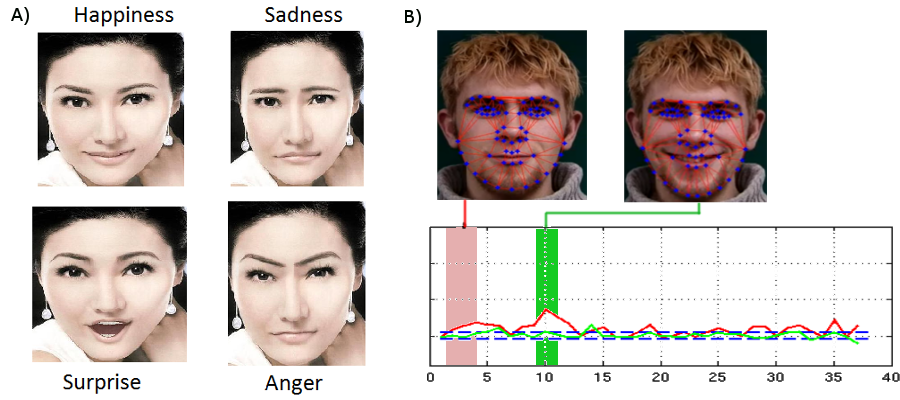
\includegraphics[scale=0.4]{images/emotionsAndGraphics1.png}
    \caption[Basic human emotions and Facial gesture analysis]{(A) Basic human emotions. (B) Facial gesture analysis. Emotion is a complex psychophysiological experience of an individual's state of mind as interacting with biochemical (internal) and environmental (external) influences}
    \label{fig:BasicEmotions}
\end{figure}

In computer vision and artificial intelligence (AI) there are many sub-problems related to facial emotion recognition such as: pose variations, people constantly moving their head in different angles; illumination changes, different environments with different illumination conditions; occlusion, which occurs when an object is in front of the face difficulting the analysis feature extraction task; background complexity, multiple objects in the environment with non-uniform background contrast; finally, image resolution which affects the accuracy of the tracking/recognition process. Besides, from the computational point of view, this problem implies the classification of facial motion or facial structure deformation into abstract representations completely based on visual information.

\subsubsection{Basic concepts}

Computational facial analysis methods can be classified in deformation extraction methods and motion extraction methods \cite{Fasel01}:
\begin{description}
\item[Motion extraction:] these approaches focus on facial changes presented as consequence of facial expressions.
\item[Deformation extraction:] these approaches work with a neutral face images or face models for extract relevant facial features not caused by wrinkles or accidents.
\end{description}

The main difference between them is that deformation-based methods can be applied to image sequences, in the second case, the analysis can be applied to both single images and image sequences by processing frames independently. However, deformation-based feature extractors miss low-level directional motion information, i.e. they cannot reconstruct pixel motion. Although face motion can be inferred by using facial feature models it requires extra computation time to achieve it.

In both cases, facial features may be processed holistically (the faces are analyzed as a whole) or locally (focusing on features from specific areas).These approaches are focused on the extraction and analysis of two types of facial features \cite{Fasel01}:
\begin{description}
\item[Intransient facial features:] always are in the face and could be deformed by facial expressions, for example, eyes, eyebrows and mouth.
\item[Transient facial features:] consider wrinkles and bulges in the face, for example, when the people open and close their eyes or mouth, face changes.
\end{description}

In both cases, the success of the technique depends on the capacity to segment the face from background. The correct segmentation allows an accurate extraction of points of interest from the faces. To do it, facial processing may take place either holistically, or locally, by focusing on facial features or areas that are prone to change with facial expressions. The task of separating the face from the background is done through segmentation, which allows the isolation of transient and intransient features within the face, that can be used to separate faces of interest from the background.

\subsubsection{Facial gestures analysis methods}
Facial gesture analysis is a challenging task and it has several application related to human interaction and computers. Traditionally, facial gestures recognition classifies the expressions into seven general emotions (anger, happiness, fear, sadness, contempt, disgust, surprise), in contrast, the facial expression analysis involves the reconstruction of facial motion, considering this way the facial muscle periods of motion between one gesture and another. In this cases it is necessary a robust classification and tracking technique of face gestures and head position \cite{Cinar01}.

There are three main steps for working in facial gestures recognition: face detection, extraction of facial gestures information and classification of the information extracted. As it was previously stated, the methods for facial gesture analysis can be grouped in deformation extraction and motion extraction.% (see Tables \ref{tb:Deformation} and \ref{tb:Motion}).

\begin{comment}
\subsubsection{Deformation extraction}
This type of methods are characterized by shape and texture changes and tendency to high spatial gradients that are good indicators for facial actions and may be analyzed either in the image or the spatial frequency domain.
The latter can be computed by techniques like Gabor wavelet-based filters, which closely model the receptive field properties of cells in the primary visual cortex \cite{Daugman1}.

These techniques are divided in three groups:

\begin{itemize}
\item Holistic image-based approaches.There are a considerable number of authors that have worked with whole faces as features. Most of them use 2D images as input so they cannot infer depth-based information. For example, some researches have been inspired in the behavior of the simple cells in the visual cortex and they model the face with Gabor wavelets \cite{Choi}. %This method present better results in many aspects from earlier work \cite{Xiaohua2009, Lai2005}.
\item Holistic Model-based approaches. Are an alternative to image-based deformation extraction. The main characteristic of these types of methods are that allow separate and process different information sources like illumination and deformation changes. Faces are analyzed by two different approaches: Active Shape Model (ASM) \cite{Wan01} and Active Appearance Model (AAM)%\cite{Lee2009}
, this helps to determinate shape, scale and pose by fitting an appropriate point distribution model to the object of interest. Other authors have decided combine Gabor filters and AAM, as a result, this techniques can lead to more accurate matching when condition changes \cite{Gao}.
\item Local image-based approach. These techniques extract facial features from windows placed around regions of the face (one or both eyes, mouth, etc.) and are used for analysis or specific purposes. New strategies are being developed
%\cite{Zhang01, Abate2007}
, for example, face recognition based on the multi-scale local structures of the face \cite{Geng01} image where the focus is in contribute to all major steps in the feature extraction and image matching, this strategy search for the nearest subject and a two-stage image matching scheme are developed for the face identification task.
\end{itemize}

%-------------------------------------------------- TABLE 1 -----------------------------------------------------------------------------------------
\begin{table}[h]
\scriptsize
%\footnotesize
\begin{center}

\begin{tabular}{|p{4.0cm}|p{4.0cm}|p{4.0cm}|} \hline \hline
\normalsize{\bf Deformation extraction} & \normalsize{\bf Holistic methods} & \normalsize{\bf Local Methods} \\  \hline \hline
\normalsize{ Image-Based}  &  \normalsize{Gabor wavelets \cite{Kruger2002}}   & \normalsize{Multi\-scale local image structures \cite{Geng01}} \\ \hline
\normalsize{ Model-based } &  \normalsize{Active Appearance Model \cite{Cootes2002}} & \\ \hline \hline
\end{tabular}
\end{center}
\caption{Holistic and local methods for deformation extraction}
\label{tb:Deformation}
\end{table}

It is important to remark that most of the techniques found in this category uses 2D images as input. Some techniques uses explicit geometry of the face to reconstruct it or to infer depth (AAM).

\subsubsection{Motion Extraction}
These types of methods have been commonly used for the task of facial expressions analysis extracting features of the face of images sequences;there are applications about it, for example in surveillance, motion capture, image stabilization or feature tracking for 3D reconstruction.

\begin{itemize}
\item Holistic dense optical flow. Is used when is necessary analyze whole faces, when is presented motion of objects. This type of techniques can be in real time or non-real time using video databases. Other techniques implement dense optical flow map \cite{Tagliasacchi2007} trying to be more efficient, fast and making use of the minimum computational cost. 3D optical flow models is other technique and  is derived from a straightforward extension of the 2D Horn–Schunck model and discretized using standard finite differences. %\cite{elMostafa}.
\item Holistic motion models.A 3D model is used mainly to be precise to enhance the facial expression recognition or face recognition. Markov models are widely employed to recognize faces or expressions  \cite{Wang01}. Kalman filter is important in this type of techniques due to its ease and accuracy in motion and recognition of objects, in this case, faces and expressions.% \cite{Motai2012}.
\item Local motion models. Over the last years, 3D face models have been widely used in many applications, for example, face recognition, facial animation and facial expression analysis. 3D Morphable model(MMs) have become a popular tool to build and fit 3D face models to images \cite{mora}.%, Levine2009}.
\item Feature point tracking.In this techniques, motion estimates are obtained when a set of features are  selected of the face (lips, nose, eyes, etc.) Is important to note, in this techniques is important that environment is clear and have good illumination, those factors between others reduce the risk of tracking loss. There are strategies that present a different approaches about that, showing a drift-correcting template update trying to have more precision for tracking a feature point in 2D \cite{Peng}. This method has a more sustained ability to track a feature point than other previous strategies.
\end{itemize}

%-------------------------------------------------- TABLE 2 -----------------------------------------------------------------------------------------
\begin{table}[h]
\scriptsize
%\footnotesize
\begin{center}

\begin{tabular}{|p{4.0cm}|p{4.0cm}|p{4.0cm}|} \hline \hline
\normalsize{\bf Motion extraction} & \normalsize{\bf Holistic methods} & \normalsize{\bf Local methods} \\  \hline \hline
\normalsize{Dense optical flow}  &  \normalsize{Dense flow fields \cite{Holte01}}  & \normalsize{Flow-based facial expression \cite{Sanchez01}}  \\ \hline
\normalsize{Motion models}  &  \normalsize{3D motion models \cite{Urtasun2006}} & \normalsize{3D Morphable Model \cite{Vetter01}} \\ \hline \hline
\normalsize{Feature point tracking}  &   & \normalsize{Eigenface augmented \cite{Yuki01}} \\ \hline \hline
\normalsize{Difference-images}  &  \normalsize{Holistic diff. images \cite{GarciaMartinez2012}} &  \\ \hline \hline
\end{tabular}
\end{center}
\caption{Holistic and local methods for motion extraction}
\label{tb:Motion}
\end{table}
\end{comment}

\subsubsection{Review of Deformation and Motion Extraction Methods}
Over last years researchers have developed many approaches and models for face recognition and analysis with good results by using both deformation and motion extraction approaches. Although, the election of an specific technique relies on the characteristics of a certain problem. Deformation extraction have been successfully used to solve emotion recognition tasks, since they can be used to analyze single images. However, if the problem consists in analyzing a sequence of images to extract the \emph{motion} (caused by muscles actions) of different regions in the face while making a gesture, the motion extraction techniques are ideal to this goal, since they have been applied to evaluate the motion produced in areas like eyes or mouth, by using a model generated a priori.

In general, motion techniques uses either 2D or 3D information. Typically, 2D based techniques are more used due to their fastness, product of a reduced dimensionality of the information. Nevertheless,  a very large training data sets is needed to model the angular variations and illumination changes. In the case of 3D based approaches, the accuracy reached is higher than 2D based ones \cite{Fang2012}, since they are rotation invariant, although their sensitiveness to illumination changes remains.% \cite{Stratou2011}.

In the case of facial expression analysis, precision is more important than processing speed, since the analysis can be carried on offline. Considering that, 3D based techniques are more relevant to solve the problem; especially those approaches with local oriented processing, since they allow analyzing information from specific points in the face (opposed points in the face are required in order to analyze the symmetry).

\subsubsection{3D based local analysis techniques}
As it was previously stated, the main difference about these techniques is the way they process information. Holistic approaches considers the whole image to extract motion vectors, which could be used for extracting general information about the motion of the face; still to increase the accuracy of facial expressions analysis requires the motion interpretation of specific regions in the face. On this line, there are several techniques in the state of the art (see Table \ref{tb:3DLocalTechniques}) that focuses on specific regions in the face:

\begin{table}[h]
\scriptsize
%\footnotesize
\begin{center}
\begin{tabular}{||p{2.7cm}|p{2.0cm}|p{2.0cm}|p{2.0cm}|p{1.5cm}|p{1.5cm}|p{1.5cm}||} \hline \hline
Reference & Sequences & Landmarks & Database & Expr. Types & R.P. (\%) \\ \hline \hline
\normalsize{Yin \cite{Yin2006}} & 2D + 4D & 64 semi-auto & BU-3DFE & 6 & 80.2 \\ \hline \hline
\normalsize{Wang \cite{Wang2007}} & 2D + 3D & 58 auto & Private & 4 & 83.0 \\ \hline \hline
\normalsize{Sun \cite{SunFer2008}} & 2D + 4D & 83 auto & BU-4DFE & 6 & 80.9 \\ \hline \hline
\normalsize{Rosato \cite{Rosato2008}} & 2D + 4D & 22 auto & BU-3DFE, BU-4DFE & 7 & 80.1 \\ \hline \hline
\normalsize{Zhao \cite{Zhao01}} & 2D + 3D & 19 manual & Bosphorus & 7 & 94.2 \\ \hline \hline
\normalsize{Tsalakanidou \cite{Tsalakanidou2010}} & 2D + 4D & 81 auto & Private & 5 & 85.0 \\ \hline \hline
\end{tabular}
\end{center}
\caption[Methods for $3D/4D$ Facial Expression Analysis]{Methods for $3D/4D$ Facial Expression Analysis (\footnotesize{Headers: \textbf{Sequences} denotes the dimensions of the images where 2D denotes whether the method makes use of the 2D texture associated with the 3D data and 4D denotes whether the method uses temporal information from a sequence of 3D data; \textbf{Database} denotes the database from which a subset was selected; \textbf{R.P.} denotes reported performance, which is the average recognition rates}).}
\label{tb:3DLocalTechniques}
\end{table}

\begin{comment}
\begin{itemize}
\item Sun et al. \cite{SunFer2008} designed a methodology for facial expression recognition (FER) considering 3D images. They propose a spatio-temporal expression analysis approach based on a new modality, 3D dynamic geometric facial model sequences, to tackle the FER problems. This approach integrates a 3D facial surface descriptor and Hidden Markov Models (HMM) to recognize facial expressions. To study the dynamics of 3D dynamic models for FER, have been investigated three types of HMMs: temporal 1D-HMM, pseudo 2D-HMM (a combination of a spatial HMM and a temporal HMM), and real 2D-HMM.

\item Rosato et al. \cite{Rosato2008} developed an effective approach to automatically establish vertex correspondences for feature registration, and further classify facial models to specific expressions in 3D facial images. Their technique also has the hability for 3D facial expression labeling, registration, tracking, and categorization. According to the authors, one of the major obstacles for analyzing such data is lack of correspondences of features (or vertices) due to the variable number of vertices across individual models or 3D model sequences. In this work they also describe a 3D facial expression databases created with 3D facial range models of the face created with static range scanners.

\item Tsalakanidou et al \cite{Tsalakanidou2010} developed a technique for automated facial action and facial expression recognition system using 2D+3D images recorded in real-time by a structured light sensor. It is based on local feature tracking and rule-based classification of geometric, appearance and surface curvature measurements. Also conducted some experimentos under relatively non-controlled conditions demonstrate the accuracy and robustness of the approach.

\item Yin et al. \cite{Yin2006} developed an automatic techniques for 3D expression model analysis by tracking and classification mechanisms. For this, they analyze the face surface as a three dimensional timevarying 'wave', which is associated with the movement of facial expressions. They found that by tracing the behavior of the 3D primitive features precious information about the nature of the underlying physical process could be revealed. This investigation propose to study the intensity-variant facial expressions in a 3D space.

\item  Wang et al. \cite{Wang2007} developed a methodology for analyzing the facial images of schizophrenic patients by combining 2D and 3D information. The main difficulty of this type of patients is that they usually have impaired expressions in the form of 'flat' or inappropiate affects, which make the quantification of their facial expressions a challenging problem. To solve this problem the authors propose the extraction of features that includes 2D and 3D geometric features, and the moment invariants combining both 3D geometry and 2D textures.

\item Zhao et al.  \cite{Zhao01} proposed a methodology for extracting the facial action units (specific deformable regions in the face like the nostrils). Action units deform facial appearance simultaneously in landmark locations and local texture as well as geometry on 3D faces, so it is necessary to extract features from multiple facial modalities to characterize these deformations comprehensively. In order to fuse the contribution of the discriminative power from all features efficiently, authors propose to use a extended statistical facial feature models (SFAM) to generate feature instances corresponding to AU class for each feature. Then the similarity between each feature on a face and its instances are evaluated so that a set of similarity scores are obtained.
\end{itemize}

Albeit some authors that opted to create their own data bases of images/sequences there are some public data bases that offers a good reference point to evaluate the performance of our application, some of them are shown in table \ref{tb:Databases}:

\begin{table}[h]
%\scriptsize
\footnotesize
\begin{center}
\begin{tabular}{||p{2.7cm}|p{2.0cm}|p{2.0cm}|p{2.0cm}|p{1.5cm}|p{1.5cm}||} \hline \hline
Database & Subjects & Samples per subject & Total images & Expressions & Poses \\ \hline \hline
\normalsize{BU-3DFE  \cite{Lijun2006}} & 100 & 25 & 2500 & 6 expressions & n/a \\ \hline \hline
\normalsize{BU-4DFE \cite{Lijun2006}}& 101 & 6 & 606 & 6 expressions & n/a \\ \hline \hline
\normalsize{Bosphorus \cite{Savran2008}} & 105 & 31-54 & 4652 & 6 expressions & 13 pitch, yaw, and cross rotations \\ \hline \hline
\normalsize{York-3DFace \cite{Heseltine2008}} & 350 & 15 & 5250 & 5 expressions & Uncontrol led up and down \\ \hline \hline
\end{tabular}
\end{center}
\caption[Public images databases]{Public images databases and their statistics}
\label{tb:Databases}
\end{table}

\end{comment}

The approaches described previously have the ability to perform facial expressions analysis considering 3D information. These techniques can be classified into two main groups, depending on the labelling mechanism: automatic and manual. In the case of the automatic labelling mechanisms, authors have used automatic fitting techniques to extract different numbers of facial regions of interest (22- \cite{Rosato2008} and 58 \cite{Wang2007}). In the case of the manual labelling mechanisms, the existing techniques require off line characterization of the facial regions of interest. As it can be seen in Table \ref{tb:3DLocalTechniques}, there is a difference on the percentage of recognition achieved by techniques in these two categories: methodologies designed to manual labelling reached as top a 94.2\% compared to 85.0\%. Also from the table \ref{tb:3DLocalTechniques}, there is no clear difference about the number of points to be used (but the higher the number of points is the higher computational complexity as well as a higher recognition rate). Although it remains to review, automatic labelling techniques are more desirable for facial expression analysis problems, since they reduce the dependance from user interaction.
%Even though there are some functional commercial applications they need to stablish some restrictions to obtain higher recognition rates and are more oriented to emotion recognition rather than facial expression analysis, as it can be seen in the following.

\begin{comment}

\subsection{Commercial software}
\label{Sec:ComSoft}

There are different software for facial expression recognition, but none is 100\% effective. One of them is {\bf faceAPI \cite{faceApi2}} that allows  to incorporate Seeing Machines world class face tracking technology into one product or application. faceAPI provides a suite of image-processing modules created specifically for tracking and understanding faces and facial features. Seeing Machines faceAPI is the only comprehensive, integrated solution for developing products that leverage real-time face tracking. All image-processing for face tracking is handled internally, removing the need for any computer vision experience. \\

The features of this software are:
\begin{itemize}
\item Highly robust, real-time, automatic monocular 3D face tracking.
\item Tracks head-position in 3D providing X,Y,Z position and orientation coordinates per frame of video.
\item Tracks 3 points on each eyebrow and 8 points around the lips.
\item Pose-normalized face texture output, annotated with facial feature coordinates.
\item Can track up to +/- 90 degrees of head rotation.
\item Robust to fast movements, large head rotations, lighting, facial deformation, skin color, beards, glasses etc.
\end{itemize}

\begin{figure}[H]
    \centering
    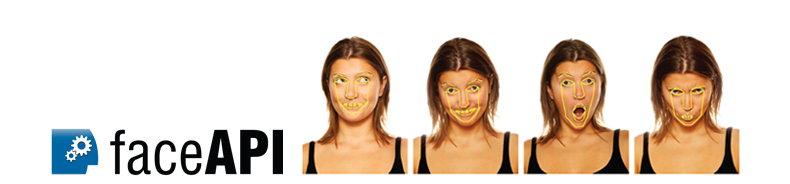
\includegraphics[scale=0.5]{faceapi.png}
    \caption{faceApi software.}
    \label{fig:faceApi software}
\end{figure}

{\bf Affdex} \cite{affdex2}is other commercial software for facial expressions recognition. Affdex reads emotional states such as surprise, dislike and attention from facial expressions using a web cam. It employs advanced computer vision and machine learning techniques to recognize and automate the analysis of tacit expressions, and it applies scientific methods to interpret viewers' emotional responses quickly and at scale. \\

The main features of this software are:
\begin{itemize}
\item Affdex integrates seamlessly into an existing survey process from measurement through insight. This includes the Affdex dashboard, where survey results are combined with Affdex emotional analysis for more power insights, faster.
\item Affdex unleashes the power of cloud computing coupled with a simple web cam to easily and cost-effectively reach more people, in more places.
\item Automatic segmentation analysis through survey integration.
\end{itemize}

\begin{figure}[h]
    \centering
    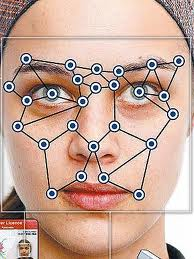
\includegraphics[scale=0.5]{facialExpression1.jpg}
    \caption{Affdex software.}
    \label{fig:Affdex software}
\end{figure}

Though, there disadvantages in this type of software, for example:
\begin{itemize}
\item They are not tolerant to occlusion.
\item Their accuracy decreases when illumination is low.
\item They can not determine whether the emotion is feigned.
\item they only can recognize specific expressions, cannot be trained.
\end{itemize}


Considering the reviewed information about different techniques for human facial expression analysis we state the problem and research questions in the next section.
\end{comment}
